\documentclass[UTF8,aspectratio=169]{ctexbeamer}
\usetheme{Madrid}
\usecolortheme{default}
\usepackage{amsmath}
\usepackage{booktabs}
\usepackage{siunitx}
\usepackage{graphicx}
\usepackage{array}
\usepackage{xcolor}
\usepackage{xurl}

\graphicspath{{assets/}}
\newcommand{\good}[1]{\textcolor{green!45!black}{#1}}
\newcommand{\warn}[1]{\textcolor{red!65!black}{#1}}
\newcommand{\bluenote}[1]{\textcolor{blue!65!black}{#1}}
\newcommand{\src}[1]{\vfill{\tiny\textcolor{gray!75!black}{Source: \url{#1}}}}
\newcolumntype{L}[1]{>{\raggedright\arraybackslash}p{#1}}
\newcolumntype{R}[1]{>{\raggedleft\arraybackslash}p{#1}}

\title[MLP Probabilistic Calibration]{Probabilistic Calibration for MLP Uncertainty\\ \small Beyond Deterministic Spray Baselines}
\author{Mie Spray Postprocessing Project}
\date{\today}

\begin{document}

\begin{frame}
  \titlepage
\end{frame}

\begin{frame}{The Core Argument}
\textbf{Goal:}
Prove that the MLP not only predicts accurate mean penetration trajectories but also provides \textbf{statistically reliable dynamic uncertainty bounds ($\sigma$)}. 

\vspace{0.5em}
\textbf{The Limitation of Traditional Baselines:}
\begin{itemize}
    \item Physical baselines (Hiroyasu-Arai, Naber-Siebers) are fundamentally \textbf{deterministic}.
    \item They predict a point estimate, but any provided error boundaries are usually just static, globally computed historical residuals.
    \item They cannot dynamically adjust confidence based on the instantaneous out-of-distribution (OOD) nature of the specific injection condition.
\end{itemize}

\vspace{0.5em}
\textbf{The Solution:} We upgrade our evaluation from simple empirical coverage metrics to formal \textbf{Probabilistic Forecasting Diagnostics}.
\end{frame}

\begin{frame}{Evaluation Protocol}
\small
\begin{block}{Common clean diagnostic set}
All models are evaluated on the same \num{795561} points. For every point \(i\),
the diagnostic consumes a scalar observation \(y_i\), predictive mean \(\mu_i\),
and predictive standard deviation \(\sigma_i\).
\end{block}

\begin{block}{Why this matters}
RMSE and MAE only test \(\mu_i\). Calibration diagnostics test whether
\(\sigma_i\) is statistically meaningful: a useful uncertainty model must be
both \emph{calibrated} and \emph{sharp}.
\end{block}

\begin{block}{Models compared}
Calibrated Hiroyasu--Arai, Naber--Siebers delay, old Stage-3 MLP
\(\Delta P^{0.25}\), and five new Stage-3 MLP \(\Delta P^{0.5}\) seeds.
\end{block}

\src{MLP/eval/calibration_diagnostics.py}
\end{frame}

\begin{frame}{Metric 1: Reliability Diagram \& Expected Calibration Error (ECE)}
\small
\textbf{Step 1: convert each observation to a predictive percentile}
\[
u_i = F_i(y_i) =
\Phi\!\left(\frac{y_i-\mu_i}{\sigma_i}\right),
\]
where \(F_i\) is the predicted Gaussian CDF.

\textbf{Step 2: compare nominal and empirical lower-tail probabilities}
\[
\hat p(\alpha)=\frac{1}{n}\sum_i \mathbf{1}\{u_i\leq\alpha\},
\qquad
\mathrm{ECE}=\frac{1}{|\mathcal{A}|}\sum_{\alpha\in\mathcal{A}}
|\hat p(\alpha)-\alpha|.
\]

\vspace{0.2em}
\begin{itemize}
    \item A calibrated model lies on the identity line \(\hat p(\alpha)=\alpha\).
    \item ECE is unitless; lower is better.
    \item This is stricter than only checking 1\(\sigma\)/2\(\sigma\) coverage because it tests many probability levels.
\end{itemize}
\end{frame}

\begin{frame}{Metric 2: Continuous Ranked Probability Score (CRPS)}
\small
\textbf{Definition for a Gaussian predictive distribution}
\[
z_i=\frac{y_i-\mu_i}{\sigma_i},
\qquad
\mathrm{CRPS}_i
=\sigma_i\left[
z_i(2\Phi(z_i)-1)+2\phi(z_i)-\frac{1}{\sqrt{\pi}}
\right].
\]

\vspace{0.2em}
\begin{itemize}
    \item CRPS has the same unit as the target: millimetres here.
    \item It is a proper scoring rule: the expected score is minimized by the true predictive distribution.
    \item Lower CRPS means a better calibration--sharpness trade-off, not merely a wider interval.
    \item Sharpness is reported separately as \(\operatorname{mean}(\sigma_i)\); sharpness is good only when calibration remains acceptable.
\end{itemize}
\end{frame}

\begin{frame}{Metric 3: Probability Integral Transform (PIT) \& KS Test}
\small
\textbf{PIT values are the same percentiles used for reliability:}
\[
u_i=\Phi\!\left(\frac{y_i-\mu_i}{\sigma_i}\right).
\]
If the predictive distributions are calibrated, the set \(\{u_i\}\) should be
uniform on \([0,1]\).

\vspace{0.2em}
\begin{itemize}
    \item U-shaped PIT: too many observations fall in predictive tails, often indicating under-dispersion / overconfidence.
    \item Hump-shaped PIT: too many observations fall near the predictive median, often indicating over-dispersion / conservative variance.
    \item A one-sided skew indicates systematic bias in \(\mu\).
    \item With \(n=\num{795561}\), KS \(p\)-values become extremely sensitive; histogram shape and ECE are more informative than treating \(p=0\) as a simple failure label.
\end{itemize}
\end{frame}

\begin{frame}{Calibration Results: Summary Table}
\scriptsize
\begin{center}
{\setlength{\tabcolsep}{2.5pt}
\begin{tabular}{L{0.38\linewidth}R{0.10\linewidth}R{0.11\linewidth}R{0.12\linewidth}R{0.10\linewidth}R{0.10\linewidth}}
\toprule
Model & ECE & CRPS & Sharp. & 1\(\sigma\) & 2\(\sigma\) \\
\midrule
Hiroyasu--Arai calibrated & 0.070 & 5.503 & 7.478 & 0.536 & 0.886 \\
Naber--Siebers delay & 0.045 & 4.894 & 7.632 & 0.620 & 0.893 \\
Stage-3 MLP \(\Delta P^{0.25}\), seed 42 & \good{0.035} & 3.409 & \good{6.505} & 0.745 & 0.979 \\
\good{Stage-3 MLP \(\Delta P^{0.5}\), 5-seed mean} & 0.044 & \good{3.245} & 6.611 & 0.774 & 0.981 \\
\bottomrule
\end{tabular}
}
\end{center}

\vspace{0.35em}
\footnotesize
\textbf{Readout:} the new \(\Delta P^{0.5}\) MLP has the best CRPS, so its full
predictive distributions score best overall. It is conservative on the clean set
(coverage above 0.683/0.954), while the old seed-42 model has the lowest ECE but
worse CRPS and no five-seed aggregate.

\src{MLP/baseline/comparison_reports/calibration_20260509_215557/summary.csv}
\end{frame}

\begin{frame}{Reliability Diagram: ECE in Picture Form}
\centering
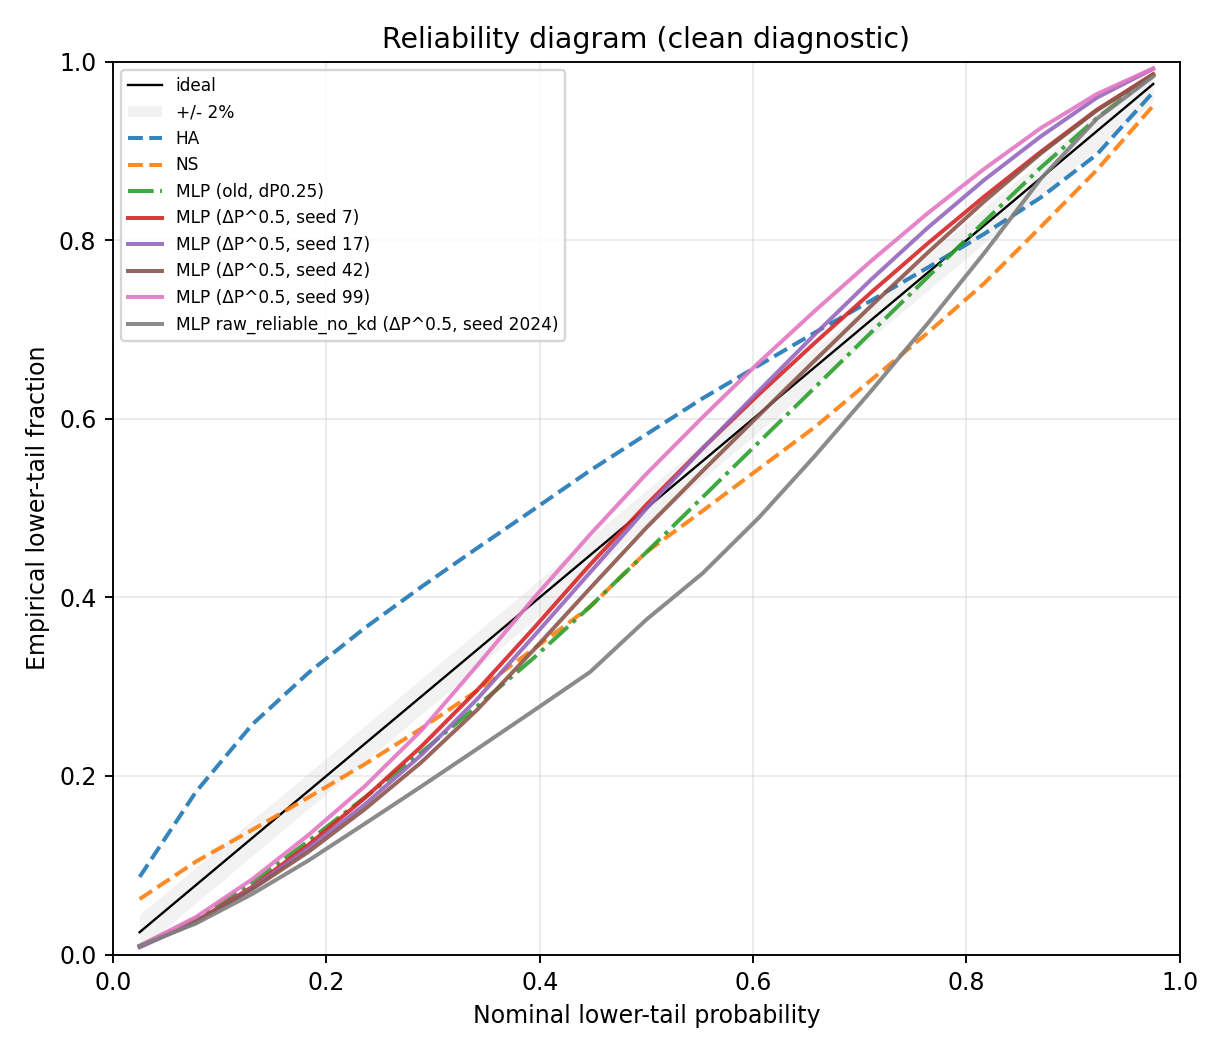
\includegraphics[width=0.78\linewidth,height=0.72\textheight,keepaspectratio]{reliability_overlay.png}

\vspace{0.15em}
\footnotesize
The diagonal is perfect lower-tail calibration. The \(\Delta P^{0.5}\) MLP family
stays closer to the diagonal than the deterministic baselines, though the seed-2024
variant visibly drives the five-seed mean ECE upward.

\src{MLP/baseline/comparison_reports/calibration_20260509_215557/reliability_overlay.png}
\end{frame}

\begin{frame}{CRPS vs Sharpness}
\centering
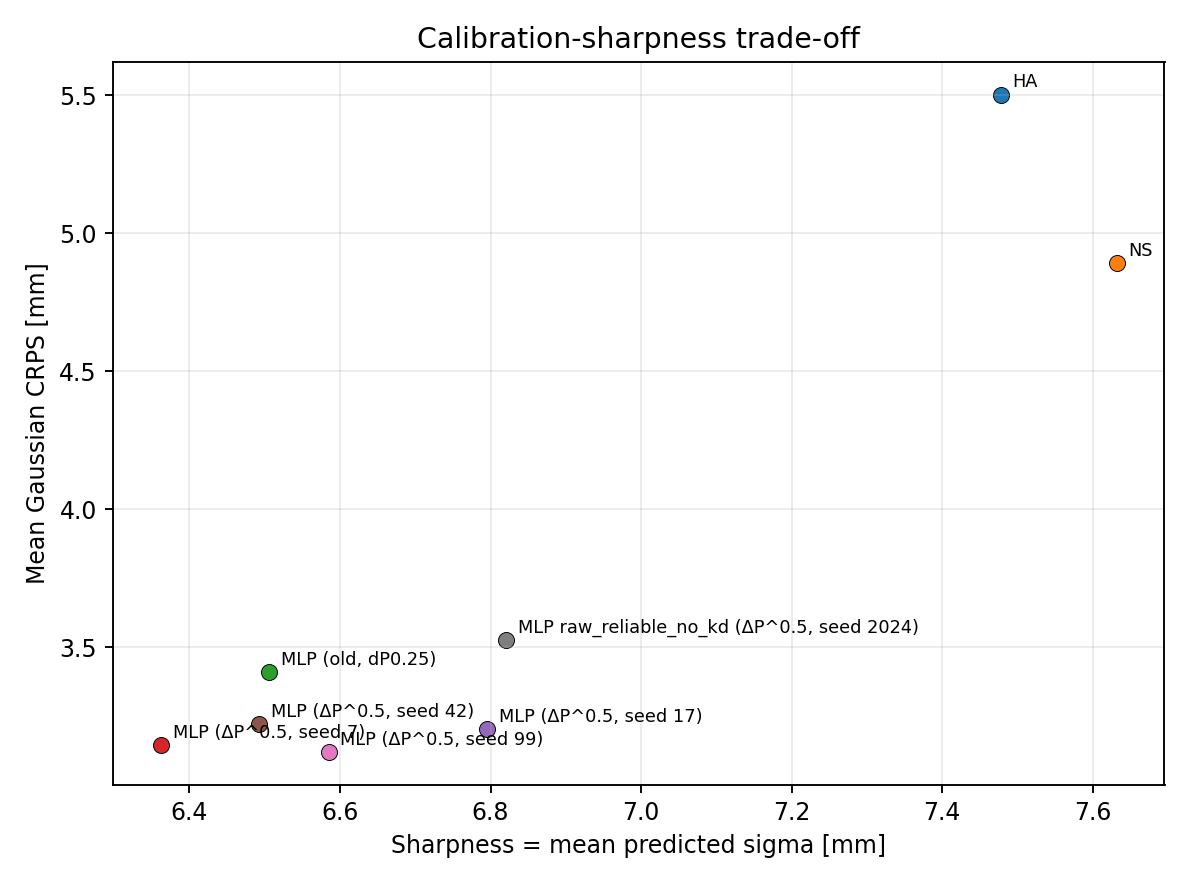
\includegraphics[width=0.82\linewidth,height=0.72\textheight,keepaspectratio]{crps_sharpness_scatter.png}

\vspace{0.15em}
\footnotesize
Lower-left is better only if reliability is acceptable. The MLP points dominate
HA/NS in CRPS at similar or lower mean \(\sigma\), showing that the improvement is
not produced by simply widening the uncertainty bands.

\src{MLP/baseline/comparison_reports/calibration_20260509_215557/crps_sharpness_scatter.png}
\end{frame}

\begin{frame}{PIT Histograms}
\centering
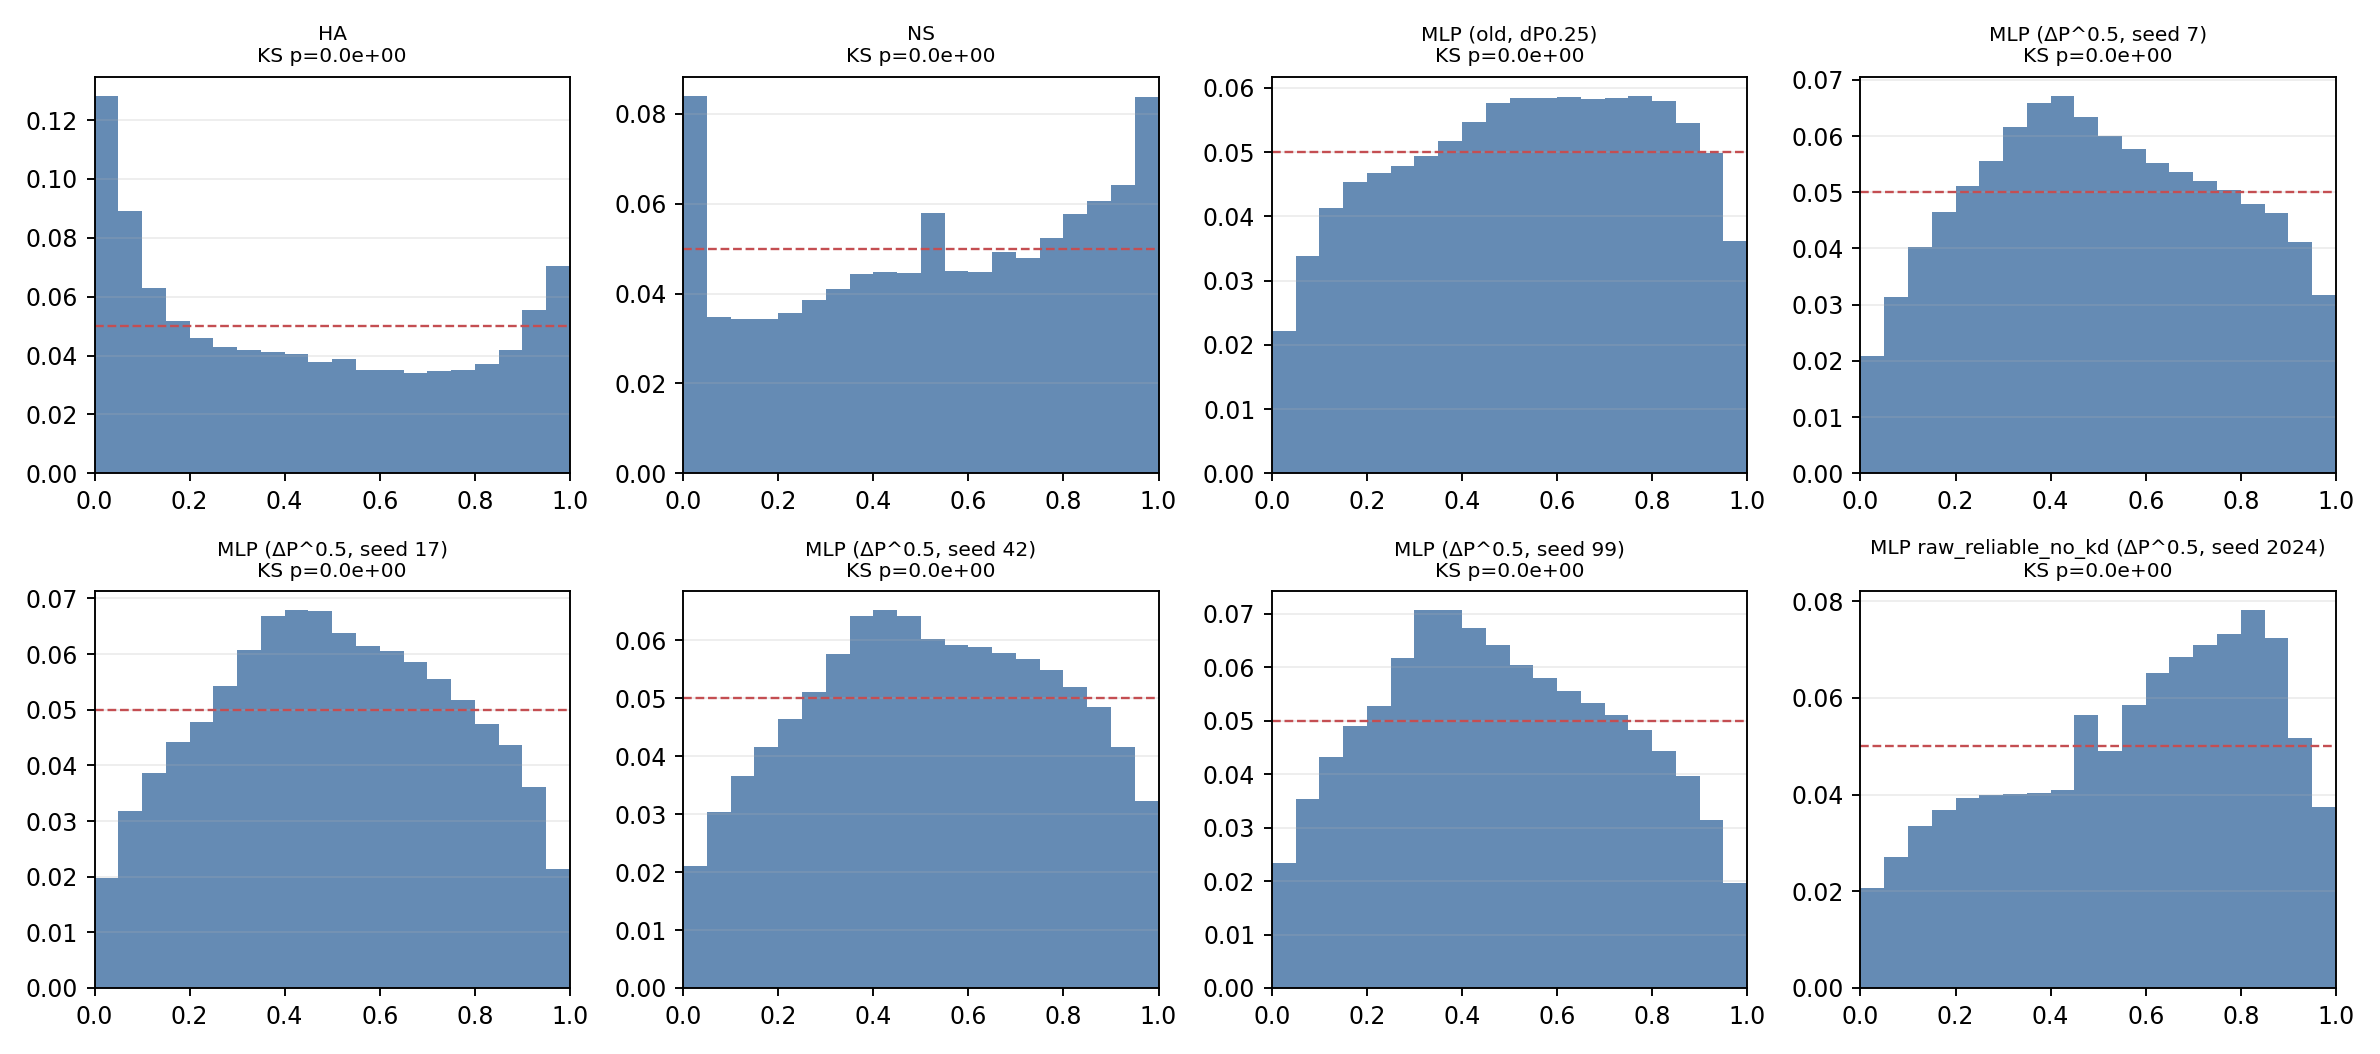
\includegraphics[width=0.94\linewidth,height=0.64\textheight,keepaspectratio]{pit_histograms.png}

\vspace{0.05em}
\footnotesize
PIT histograms diagnose the failure mode: skew means bias, U-shape means
under-dispersion, and centre-heavy histograms mean conservative variance. Because
the sample is very large, visual shape is interpreted together with ECE and CRPS.

\src{MLP/baseline/comparison_reports/calibration_20260509_215557/pit_histograms.png}
\end{frame}

\begin{frame}{Conclusion}
\textbf{Thesis Contribution:}
By integrating Reliability Diagrams, CRPS, and PIT histograms, we provide a complete suite of diagnostics (as implemented in \texttt{calibration\_diagnostics.py}). 

\vspace{0.5em}
\bluenote{\textbf{Takeaway:}}\\
Unlike Naber--Siebers or Hiroyasu--Arai models which output rigid curves plus
global residual bands, the MLP acts as a heteroscedastic probabilistic surrogate.
The current evidence is strongest in CRPS and coverage: the \(\Delta P^{0.5}\)
five-seed MLP has the best CRPS and conservative clean-set coverage, while GP-style
or deterministic baselines remain useful references for nominal calibration.
\end{frame}

\end{document}
